\documentclass[pdf]{beamer}
\usepackage{listings}
\usepackage{color}

\definecolor{dkgreen}{rgb}{0,0.6,0}
\definecolor{gray}{rgb}{0.5,0.5,0.5}
\definecolor{mauve}{rgb}{0.58,0,0.82}

\lstset{frame=none,
language=C,
columns=flexible,
numberstyle=\tiny\color{gray},
keywordstyle=\color{blue},
commentstyle=\color{dkgreen},
stringstyle=\color{mauve},
breaklines=true,
breakatwhitespace=true,
tabsize=4,
showstringspaces=false,
basicstyle=\ttfamily
}
\usepackage{parskip}
\usepackage{graphicx}
\graphicspath{{../images/}}

\mode<presentation>
{
	\usetheme{default}      % or try Darmstadt, Madrid, Warsaw, ...
	\usecolortheme{default} % or try albatross, beaver, crane, ...
	\usefonttheme{default}  % or try serif, structurebold, ...
	\setbeamertemplate{navigation symbols}{}
	\setbeamertemplate{caption}[numbered]
}

\begin{document}
\title{Intel Cloud Orchestration Networking Design and Goals}
\author{Matthew Johnson, Cody Malick, and Garrett Smith}
\date{7 December, 2016}

\maketitle
\begin{frame}
	\frametitle{Table of Contents}
	\tableofcontents
\end{frame}

\begin{frame}
	\frametitle{Team Cloud Orchestra}
	\section{Introduction}
	Our team is implementing a software defined network based on Open
	vSwitch for a cloud orchestration technology called Ciao.

	Our client is Rob Nesius, Engineering Manager at Intel Corporation.
\end{frame}

\begin{frame}
	\frametitle{Scope}
	\section{Scope}
	What is a cloud?
	\begin{figure}[H]
		\caption{The Cloud - Randall Munroe~\cite{xkcd908}}
		\begin{center}
			\makebox[\textwidth]{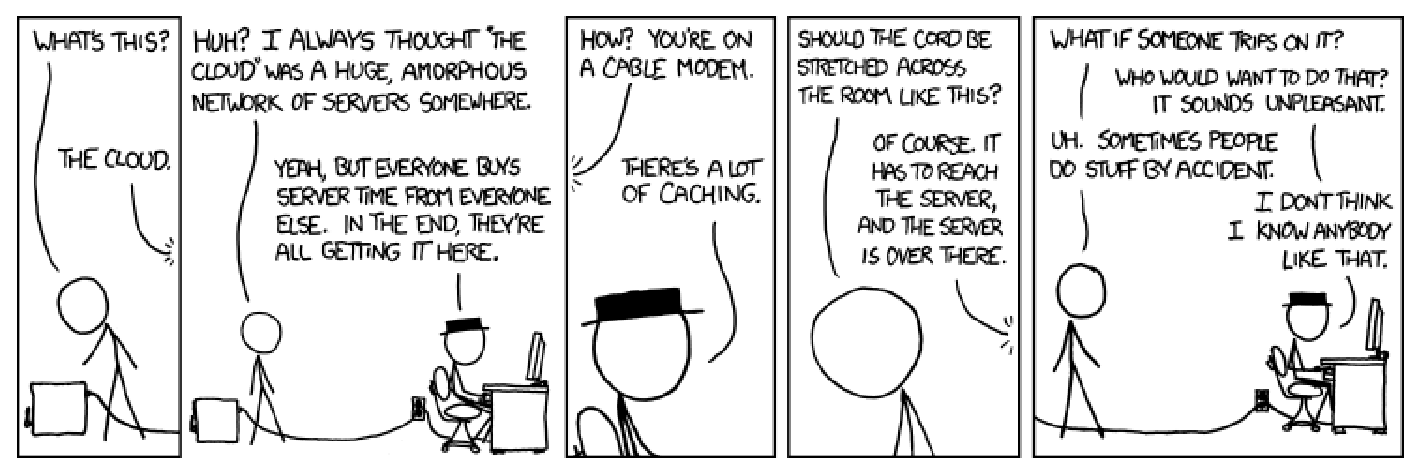
\includegraphics[width=\textwidth]{xkcd.eps}}
		\end{center}
	\end{figure}

	"A huge, amorphous network of servers somewhere"

\end{frame}

\begin{frame}
	\frametitle{Scope}
	The network connecting the nodes must be controlled. In our case, this
	is achieved by the Cloud Integrated Advanced Orchestrator, or Ciao.

	Ciao provides an easy to deploy, secure, scalable cloud orchestration
	system which handles virtual machines, containers, and bare metal apps
	agnostically as generic workloads~\cite{ciao}.
\end{frame}

\begin{frame}
	\frametitle{Scope}
	The servers, or nodes, in these clouds need to talk to each other, hence
	the need for a network solution.

	Ciao uses a software defined network to allow different compute nodes to
	communicate with each other.

	Software defined networking is a software abstraction of physical
	networking solutions, allowing for ``a more scalable and centralized
	network control architecture''~\cite{goransson}.
\end{frame}

\begin{frame}
	\frametitle{Project Goals}
	\framesubtitle{Goal One}
	\section{Project Goals}
	Switch Ciao Generic Routing Encapsulation (GRE) tunnel implementation to
	use Open vSwitch-created GRE tunnels.

	\begin{description}[style=nextline]
		\item[Generic Routing Encapsulation (GRE)]
			GRE encapsulates an arbitrary network layer protocol so
			it can be sent over arbitrary network layer
			protocol~\cite{rfc1701}.
		\item[Open vSwitch (OVS)]
			Open vSwitch is a ``multilayer virtual switch\ldots
			designed to enable massive network automation through
			programmatic extension''~\cite{ovs}.
	\end{description}
\end{frame}

\begin{frame}
	\frametitle{Project Goals}
	\framesubtitle{Goal Two}
\end{frame}

\begin{frame}
	\frametitle{Project Goals}
	\framesubtitle{Goal Three (optional)}
\end{frame}

\begin{frame}
	\frametitle{Project Design}
	\section{Open vSwitch Database Management Protocol}
	Open vSwitch uses a database to manage configuration while running.
	The configuration can be updated on the fly by accessing its management
	protocol using the Open vSwitch Database Management Protocol, defined
	in RFC 7047\cite{rfc7047}
\end{frame}

\begin{frame}[fragile]
	\frametitle{Libovsdb}
	Libovsdb is an open source library that provides a Go programming
	language wrapper around the OVS Database Management Protocol. Here is
	an example:\cite{gosample} \\

\begin{lstlisting}[caption=Example insert operation using libovsdb]
	// simple insert operation
	insertOp := libovsdb.Operation{
	    Op:	  "insert",
	    Table:	  "Bridge",
	    Row:	  bridge,
	    UUIDName: namedUUID,
	}

\end{lstlisting}
\end{frame}
\begin{frame}
	\frametitle{nvGRE and VxLAN}
	Two alternative tunneling protocols to replace GRE, the current
	protocol used by Ciao.\\
	nvGRE: Network virtualization standard created in tandem by HP, Dell,
	and Intel
	VxLAN: Network virtualization standard created in tandem by Cisco,
	VMware, Citrix, and Redhat

	Overall performance and overhead are similar on paper, will require
	testing to see which is the best fit for our implementation
\end{frame}
\begin{frame}[allowframebreaks]
	\frametitle{Stumbling Blocks}
	\section{Stumbling Blocks}
	The one major problem we had during the fall quarter was getting the 
	Intel NUCs connected to the campus network.
	We required network access to install Clear Linux on the NUCs, to access
	them remotely via SSH, and to perform actions that require internet access 
	such as accessing the Ciao git repository hosted on GitHub.
	Intel wants us to store the NUCs in a secure location. Kevin McGrath let us 
	use his lab which has restricted access.

	We set the NUCs up in Kevin's lab on campus, and had to work with Todd 
	Shecter, the head of the OSU EECS IT department to get permission to 
	connect them to the campus network, and register them so they would be able 
	to connect to the campus network. This took three weeks between technical 
	issues and communication delays because most of our communication was done 
	by email.

	\section{Network Setup Issues}
	\begin{itemize}
		\item We first emailed Todd with an explanation of our project and 
			requested network access. He requested a meeting to better 
			understand what we were doing.
		\item After explaining our project to Todd in person, he gave us 
			permission to connect the NUCs to the campus network, and said he 
			would help.
		\item To connect the NUCs to the network Todd required the MAC address 
			of each device.
		\item None of the NUCs had an OS on them, and the MAC address was not 
			listed on the case, or in the BIOS.
			We had to boot each NUC from a USB flash drive to get the MAC 
			address.
		\item We provided Todd with the MAC addresses of each NUC so they could 
			be connected to the campus network.
		\item We waited for Todd to register the NUCS on the campus network.
		\item After Todd registered the NUCs they were not being assigned an IP 
			address by the campus network.
		\item As a workaround so we could install Clear Linux we bridged the 
			network connection from Garrett's laptop to the NUCs.
		\item We emailed Todd explaining the IP address issue, and he had us go
			through several troubleshooting steps, none of which worked.
		\item Todd had us connect one of the NUCs to a different switch in the 
			lab which resolved the issue.
		\item We were going to move the NUCs over to the other switch, but it 
			took a couple of days before we had time to do this, and during 
			that time the campus network started assigning IP addresses to the 
			NUCs.
	\end{itemize}

\end{frame}

\begin{frame}
\end{frame}
\begin{frame}
	\frametitle{References}
		\bibliographystyle{IEEEtran}
		\bibliography{pres}
	\end{frame}
\end{document}
